% GNUPLOT: LaTeX picture with Postscript
\begingroup
  \makeatletter
  \providecommand\color[2][]{%
    \GenericError{(gnuplot) \space\space\space\@spaces}{%
      Package color not loaded in conjunction with
      terminal option `colourtext'%
    }{See the gnuplot documentation for explanation.%
    }{Either use 'blacktext' in gnuplot or load the package
      color.sty in LaTeX.}%
    \renewcommand\color[2][]{}%
  }%
  \providecommand\includegraphics[2][]{%
    \GenericError{(gnuplot) \space\space\space\@spaces}{%
      Package graphicx or graphics not loaded%
    }{See the gnuplot documentation for explanation.%
    }{The gnuplot epslatex terminal needs graphicx.sty or graphics.sty.}%
    \renewcommand\includegraphics[2][]{}%
  }%
  \providecommand\rotatebox[2]{#2}%
  \@ifundefined{ifGPcolor}{%
    \newif\ifGPcolor
    \GPcolorfalse
  }{}%
  \@ifundefined{ifGPblacktext}{%
    \newif\ifGPblacktext
    \GPblacktexttrue
  }{}%
  % define a \g@addto@macro without @ in the name:
  \let\gplgaddtomacro\g@addto@macro
  % define empty templates for all commands taking text:
  \gdef\gplbacktext{}%
  \gdef\gplfronttext{}%
  \makeatother
  \ifGPblacktext
    % no textcolor at all
    \def\colorrgb#1{}%
    \def\colorgray#1{}%
  \else
    % gray or color?
    \ifGPcolor
      \def\colorrgb#1{\color[rgb]{#1}}%
      \def\colorgray#1{\color[gray]{#1}}%
      \expandafter\def\csname LTw\endcsname{\color{white}}%
      \expandafter\def\csname LTb\endcsname{\color{black}}%
      \expandafter\def\csname LTa\endcsname{\color{black}}%
      \expandafter\def\csname LT0\endcsname{\color[rgb]{1,0,0}}%
      \expandafter\def\csname LT1\endcsname{\color[rgb]{0,1,0}}%
      \expandafter\def\csname LT2\endcsname{\color[rgb]{0,0,1}}%
      \expandafter\def\csname LT3\endcsname{\color[rgb]{1,0,1}}%
      \expandafter\def\csname LT4\endcsname{\color[rgb]{0,1,1}}%
      \expandafter\def\csname LT5\endcsname{\color[rgb]{1,1,0}}%
      \expandafter\def\csname LT6\endcsname{\color[rgb]{0,0,0}}%
      \expandafter\def\csname LT7\endcsname{\color[rgb]{1,0.3,0}}%
      \expandafter\def\csname LT8\endcsname{\color[rgb]{0.5,0.5,0.5}}%
    \else
      % gray
      \def\colorrgb#1{\color{black}}%
      \def\colorgray#1{\color[gray]{#1}}%
      \expandafter\def\csname LTw\endcsname{\color{white}}%
      \expandafter\def\csname LTb\endcsname{\color{black}}%
      \expandafter\def\csname LTa\endcsname{\color{black}}%
      \expandafter\def\csname LT0\endcsname{\color{black}}%
      \expandafter\def\csname LT1\endcsname{\color{black}}%
      \expandafter\def\csname LT2\endcsname{\color{black}}%
      \expandafter\def\csname LT3\endcsname{\color{black}}%
      \expandafter\def\csname LT4\endcsname{\color{black}}%
      \expandafter\def\csname LT5\endcsname{\color{black}}%
      \expandafter\def\csname LT6\endcsname{\color{black}}%
      \expandafter\def\csname LT7\endcsname{\color{black}}%
      \expandafter\def\csname LT8\endcsname{\color{black}}%
    \fi
  \fi
  \setlength{\unitlength}{0.0500bp}%
  \begin{picture}(7300.00,5520.00)%
    \gplgaddtomacro\gplbacktext{%
      \csname LTb\endcsname%
      \put(846,5700){\makebox(0,0)[r]{\strut{} \textbf{A}}}%
      \put(946,3704){\makebox(0,0)[r]{\strut{} 0}}%
      \put(946,4092){\makebox(0,0)[r]{\strut{} 0.2}}%
      \put(946,4480){\makebox(0,0)[r]{\strut{} 0.4}}%
      \put(946,4868){\makebox(0,0)[r]{\strut{} 0.6}}%
      \put(946,5256){\makebox(0,0)[r]{\strut{} 0.8}}%
      \put(1589,3484){\makebox(0,0){\strut{} 100}}%
      \put(2127,3484){\makebox(0,0){\strut{} 200}}%
      \put(2665,3484){\makebox(0,0){\strut{} 300}}%
      \put(3203,3484){\makebox(0,0){\strut{} 400}}%
      \put(176,4480){\rotatebox{-270}{\makebox(0,0){\strut{}mutual information (bits)}}}%
      \put(3876,4480){\rotatebox{-270}{\makebox(0,0){\strut{}mutual information (bits)}}}%
      \put(2140,3154){\makebox(0,0){\strut{}spike train length (s)}}%
      \put(4546,5700){\makebox(0,0)[r]{\strut{} \textbf{B}}}%
      \put(4646,3704){\makebox(0,0)[r]{\strut{}-0.2}}%
      \put(4646,4014){\makebox(0,0)[r]{\strut{} 0}}%
      \put(4646,4325){\makebox(0,0)[r]{\strut{} 0.2}}%
      \put(4646,4635){\makebox(0,0)[r]{\strut{} 0.4}}%
      \put(4646,4946){\makebox(0,0)[r]{\strut{} 0.6}}%
      \put(4646,5256){\makebox(0,0)[r]{\strut{} 0.8}}%
      \put(5836,3484){\makebox(0,0){\strut{} 12500}}%
      \put(6903,3484){\makebox(0,0){\strut{} 25000}}%
      \put(5840,3154){\makebox(0,0){\strut{}spike train length (s)}}%


      \put(846,2700){\makebox(0,0)[r]{\strut{} \textbf{C}}}%
      \put(1078,705){\makebox(0,0)[r]{\strut{} 0}}%
      \put(1078,1093){\makebox(0,0)[r]{\strut{} 0.03}}%
      \put(1078,1481){\makebox(0,0)[r]{\strut{} 0.06}}%
      \put(1078,1868){\makebox(0,0)[r]{\strut{} 0.09}}%
      \put(1078,2256){\makebox(0,0)[r]{\strut{} 0.12}}%
      \put(1689,484){\makebox(0,0){\strut{} 100}}%
      \put(2194,484){\makebox(0,0){\strut{} 200}}%
      \put(2698,484){\makebox(0,0){\strut{} 300}}%
      \put(3203,484){\makebox(0,0){\strut{} 400}}%
      \put(176,1480){\rotatebox{-270}{\makebox(0,0){\strut{}standard deviation (bits)}}}%
      \put(2206,154){\makebox(0,0){\strut{}spike train length (s)}}%

      \put(4546,2700){\makebox(0,0)[r]{\strut{} \textbf{D}}}%
      \put(4646,859){\makebox(0,0)[r]{\strut{} 0.3}}%
      \put(4646,1170){\makebox(0,0)[r]{\strut{} 0.4}}%
      \put(4646,1480){\makebox(0,0)[r]{\strut{} 0.5}}%
      \put(4646,1790){\makebox(0,0)[r]{\strut{} 0.6}}%
      \put(4646,2101){\makebox(0,0)[r]{\strut{} 0.7}}%
      \put(4778,484){\makebox(0,0){\strut{} 0}}%
      \put(5195,484){\makebox(0,0){\strut{} 10}}%
      \put(5611,484){\makebox(0,0){\strut{} 20}}%
      \put(6028,484){\makebox(0,0){\strut{} 30}}%
      \put(6445,484){\makebox(0,0){\strut{} 40}}%
      \put(6861,484){\makebox(0,0){\strut{} 50}}%
      \put(3876,1480){\rotatebox{-270}{\makebox(0,0){\strut{}mutual information (bits)}}}%
      \put(5840,154){\makebox(0,0){\strut{}$\tau$ (ms)}}%


    }%
    \gplgaddtomacro\gplfronttext{%
      \csname LTb\endcsname%
      \put(2216,2083){\makebox(0,0)[r]{\strut{}new}}%
      \csname LTb\endcsname%
      \put(2216,1863){\makebox(0,0)[r]{\strut{}old}}%

    }%
    \gplbacktext
    \put(0,3000){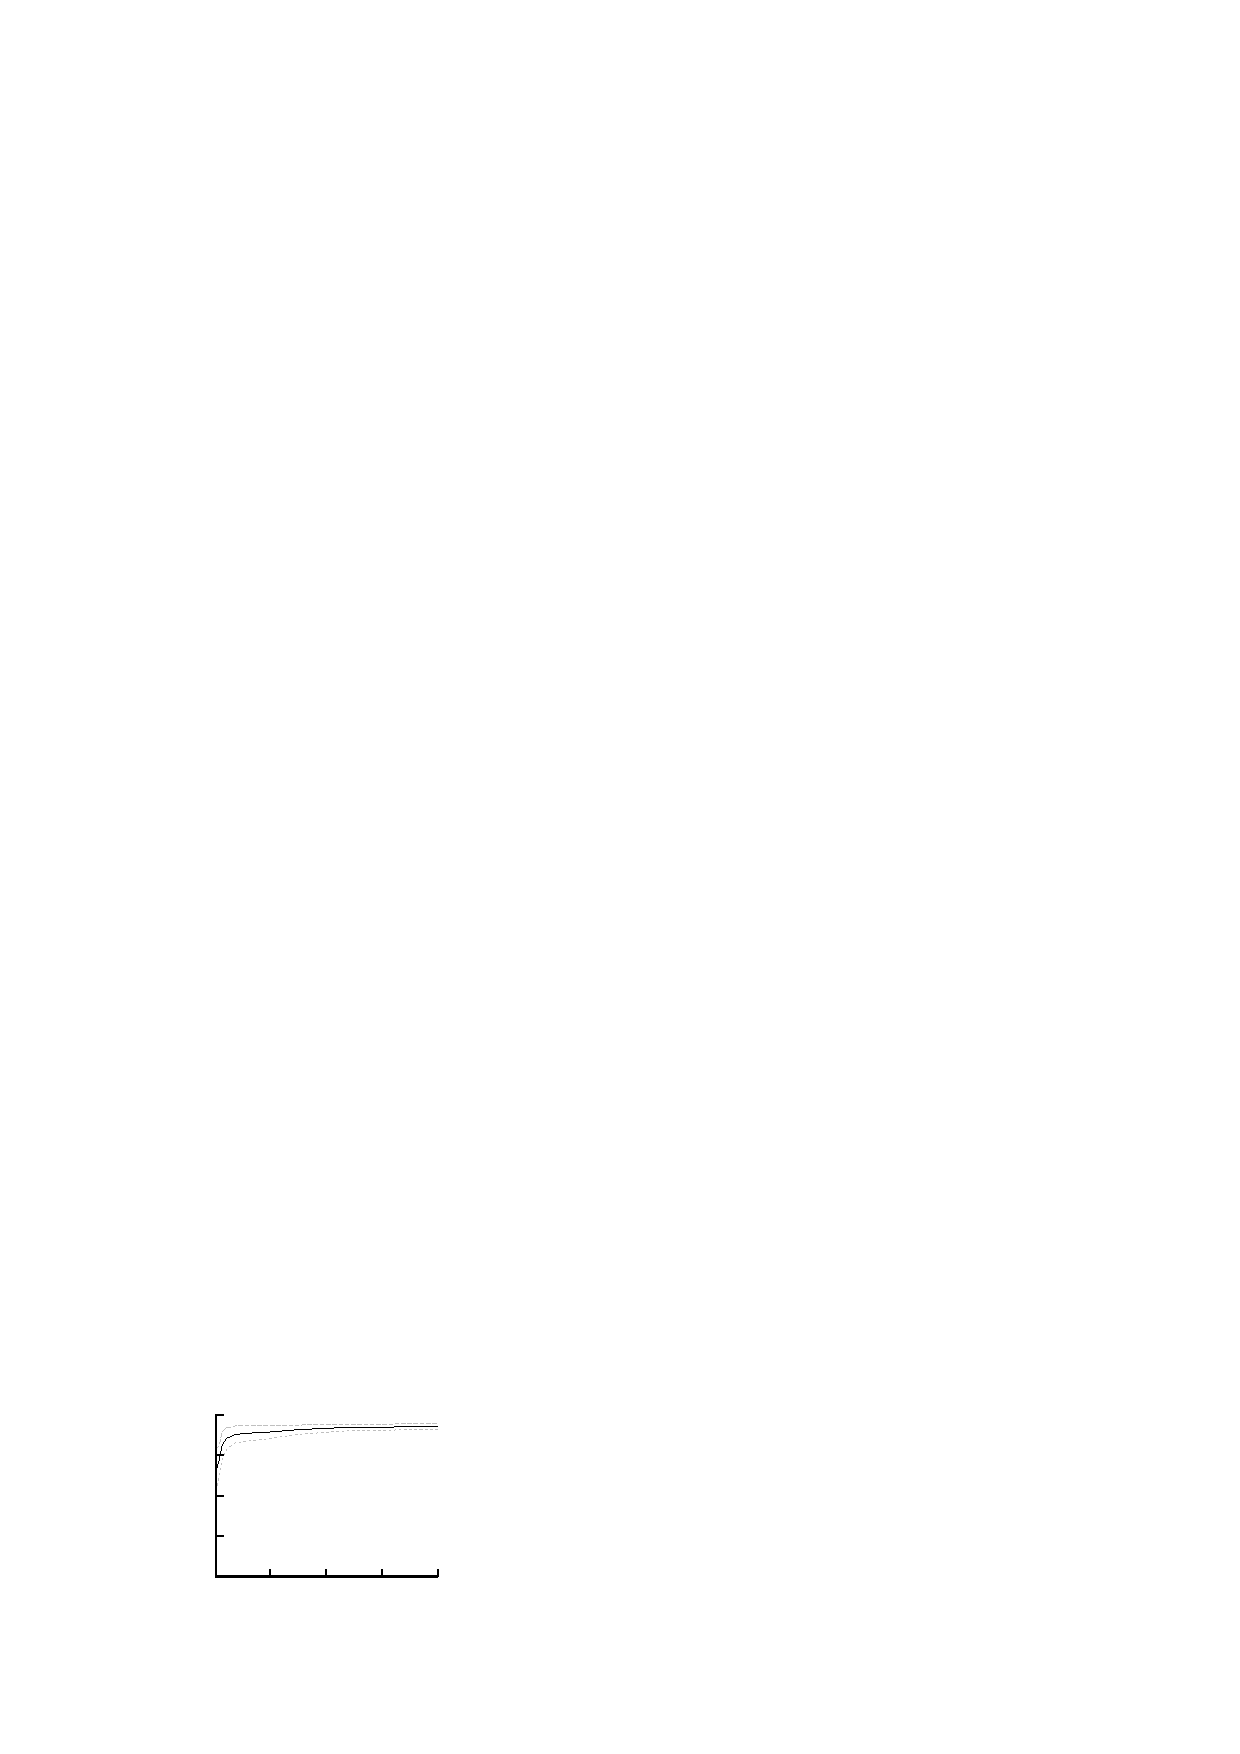
\includegraphics{length_sweep_new}}
    \put(3700,3000){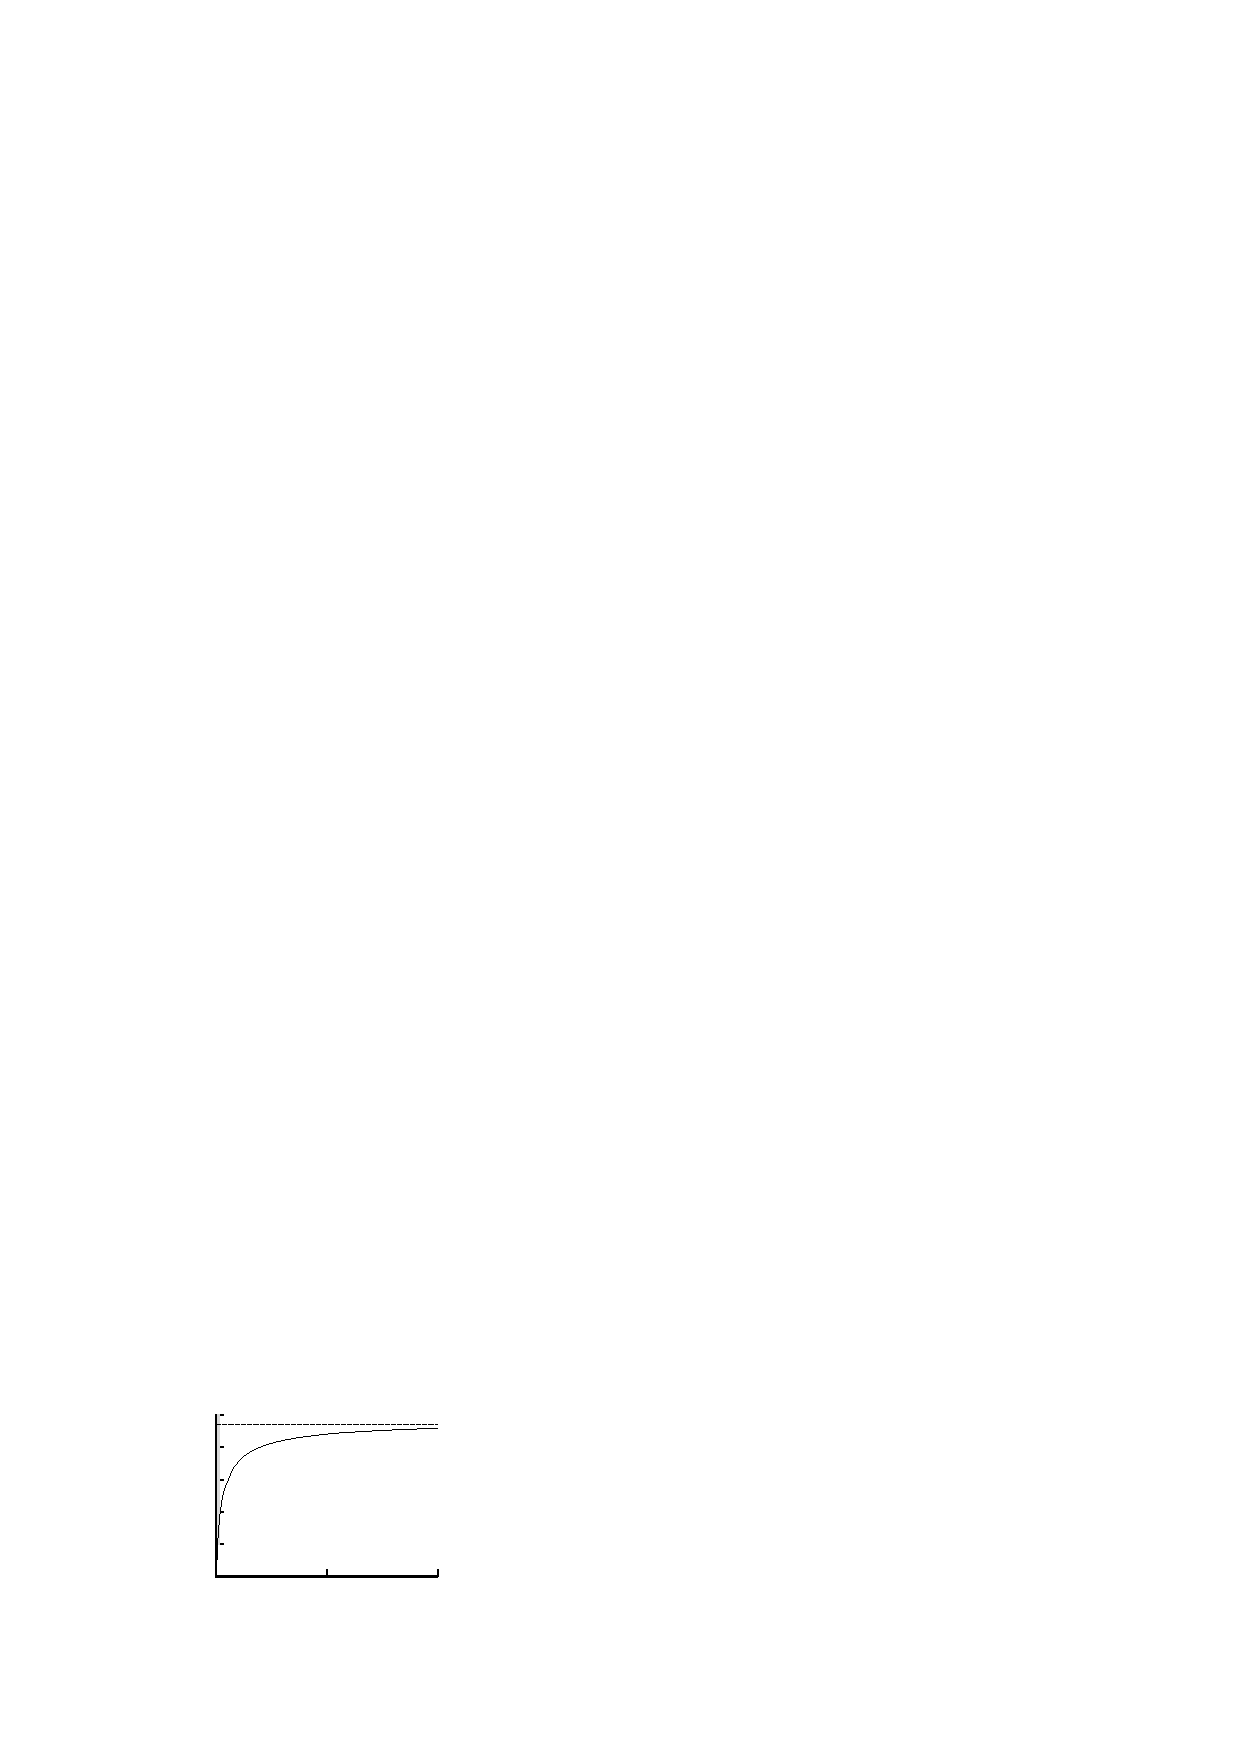
\includegraphics{length_sweep_old}}%
    \put(3700,0){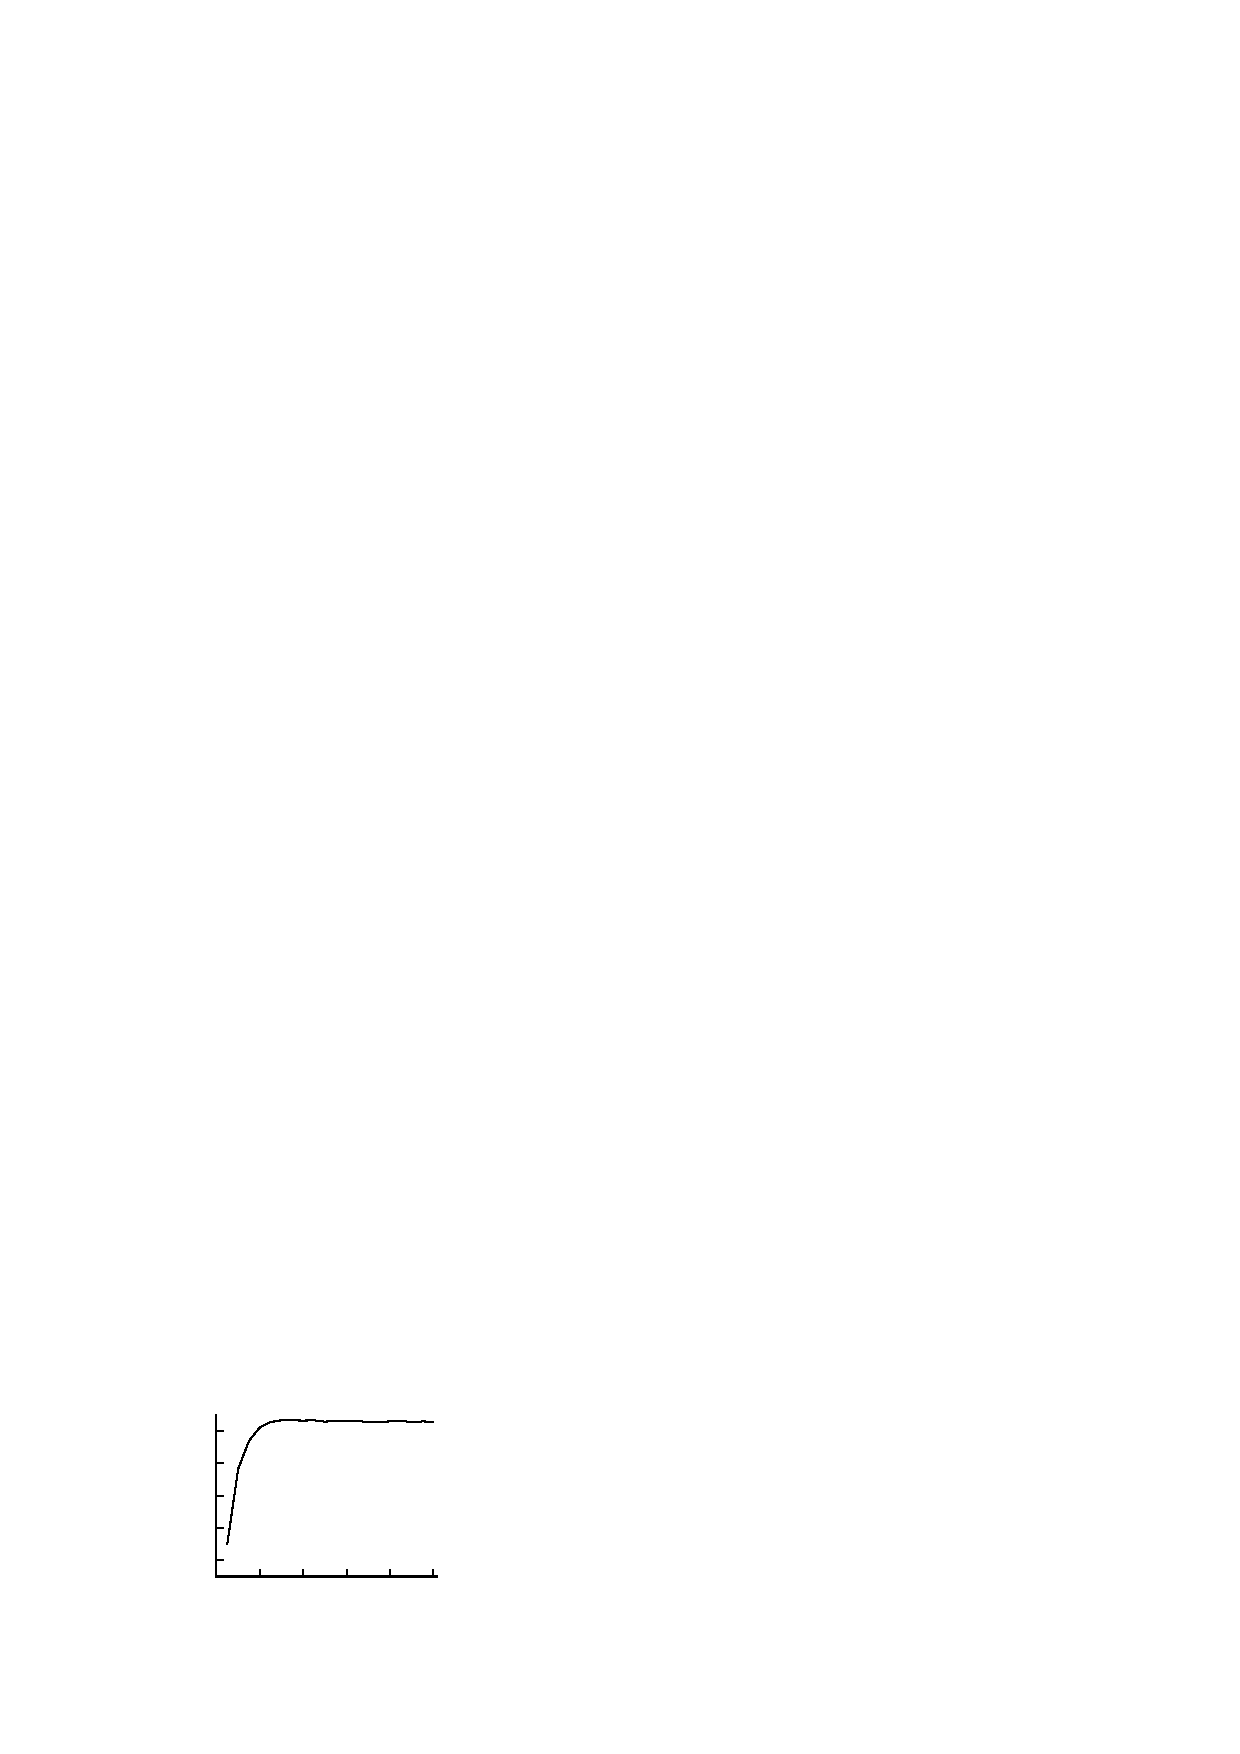
\includegraphics{fig_tau}}%
    \put(0,0){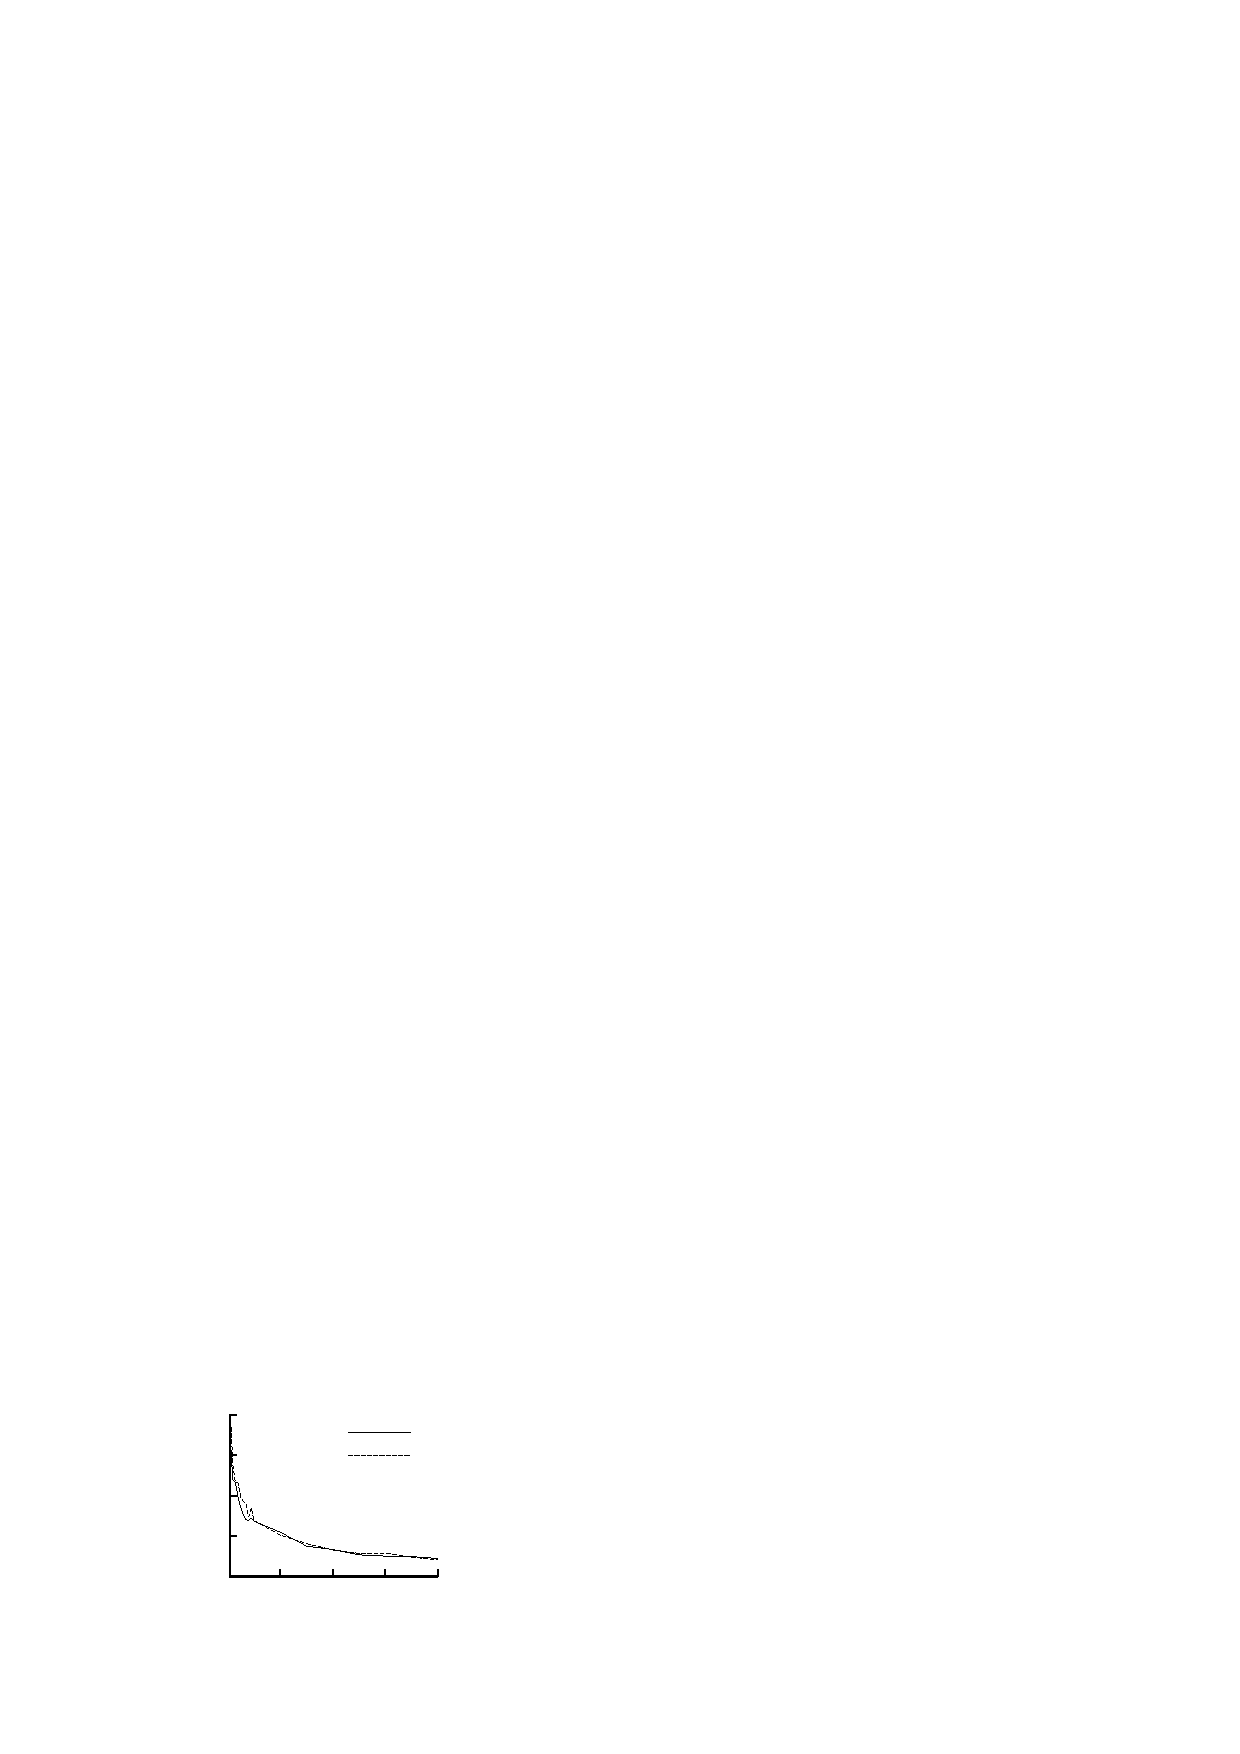
\includegraphics{fig_sd}}%
    \gplfronttext
  \end{picture}%
\endgroup
